\chapter{Implementace}

TODO: Popis implementace/realizace se zaměřením na nestandardní části řešení.

\section{Specifikace pravidel požadovaných zadáním práce}
Pro specifikaci Demeter law definujeme predikát, který nám umožní vybrat vhodné množiny vrcholů. Vybrané množiny potom ověřeíme pomocí predikátu, který učí, zda jsou tyto množiny v pořádku, či zda porušují LoD princip.

\begin{definition}
Mějme graf $G = \langle V, E, \rho, K, C, \mathit{Kind}, \mathit{Class}\rangle$ se zobrazeními definovanými dříve. Definujme selektor $F(G, v', k', c')$, $v' \in V$, $k' \in K$, $c' \in C$ jako množinu vrcholů grafu $G$, které jsou dostupné z vrcholu $v'$ pomocí orientované cesty, pro jejíž všechny vrcholy $v''$ s~výjimkou posledního platí $Kind(v) \ne k'$ a která obsahuje hranu $e$, pro niž platí $Class(e) = c' $.
\end{definition}

\subsection{Law of Demeter}
Pro provedení validace princip LoD využijeme graf podobný tomu na obrázku \ref{implementation-lod_graph}. Lze jej získat ze zdrojových kódů pogramu. Vazba $\langle\langle{}uses\rangle\rangle$ představuje všechna použití (přístup k~public a protected polím a volání metod) jiných tříd v rámci metody.

\begin{figure}[h!]
  \centering
  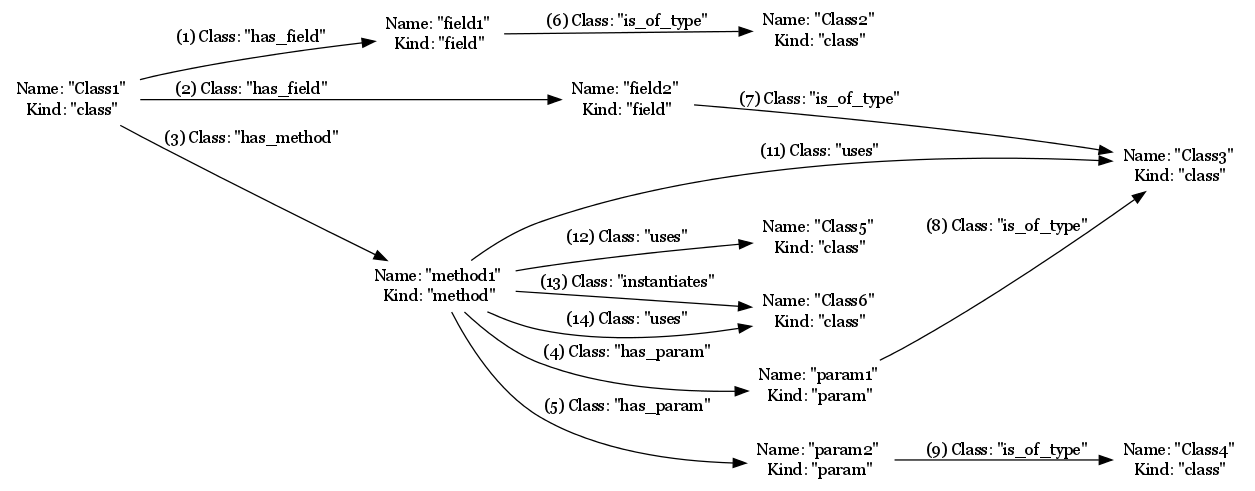
\includegraphics[width=1.0\textwidth]{./graphs/demeter_graph.png}
  \caption{Graf použitý pro validaci principu LoD.\label{implementation-lod_graph}}
\end{figure}

Pravidlo LoD potom specifikujeme nad grafem $G = \langle V, E, \rho, K, C, \mathit{Kind}, \mathit{Class}\rangle$ následovně:

\begin{align*}
\forall v \in V: Kind(v) = class\\
\end{align*}
\begin{align*}
[((&F(G, v, class, \langle\langle{}has\_field\rangle\rangle{}) \cup F(G, v, class, \langle\langle{}has\_param\rangle\rangle{}) \cup\\
&F(G, v, class, \langle\langle{}instantiates\rangle\rangle{})) \cap F(v, class, \langle\langle{}uses\rangle\rangle{}) \setminus \{v\}] = \emptyset
\end{align*}

Specifikované pravidlo vyjadřuje požadavek, aby množina vrcholů do níž se dostaneme pomocí hran, které představují povolené vstupy tříd do analyzované třídy (třídní proměnné, parametry, vytvářené objekty), byla totožná s množinou všech vrcholů, které představují všechny třídy používané (klasifikátor $\langle\langle{}uses\rangle\rangle$) v rámci některé z metod. Odečtení vrcholu $v$ z výsledné množiny je zde kvůli tomu, abychom nemuseli navíc zavádět zbytečnou hranu identifikující, že třída je známá sama sobě.

\subsection{Low coupling}
TODO:

\subsection{High cohesion}
TODO:

\section{Implementace jádra systému}
TODO: describe technologies used to implement parser and analysis part

TODO: moduly popsané v části \ref{design-architecture} implementujeme jako jednotlivé moduly platformy NetBeans.

Integrace s platformout NetBeans - třída Action.

\begin{itemize}
\item Java 6 Compiler API (JSR 199) \emph{\{TODO: add reference\}}
\item annotation processor (JSR 269) \emph{\{TODO: add reference\}}
\item Compiler Tree API
  \begin{itemize}
  \item \verb+com.sun.source.tree+
  \item \verb+com.sun.source.util+
  \end{itemize}
\end{itemize}

TODO: zapracovat:

je nutné použít nestandardní API, které je součástí Sun Javy - balíčky \verb+com.sun.*+ (je potřeba přidat \$\{java\_home\}/../lib/tools.jar do classpath)

lze se inspirovat v programu Sorcerer (\href{https://sorcerer.dev.java.net/}{https://sorcerer.dev.java.net/}), který pomocí Java Tree API provádí zpracovávání Java kódu a generování přesné HTML dokumentace. \emph{TODO: in case of usage of this material, add reference!}

\section{Implementace modulů}

\begin{itemize}
\item \emph{av-graphgen-demeter} -- ukázkový poskytovatel generátoru grafu
\item \emph{av-operators-demeter} -- ukázkový balíček operátorů pro ověřování principu LoD
\item \emph{av-reportgen-plaintext} -- ukázkový poskytovatel pro generování validačních reportů v~prostém textu
\end{itemize}

\subsubsection{GraphGeneratorManager}
Bude řídit přístup k jednotlivým graph generatorům. Umožní externím providerům registraci nových graph generátorů. Každý graph generátor (resp. graf) musí mít specifikované jedinečné id grafu. (To bude dále použito např. při specifikaci pravidel, kde je potřeba sdělit validátoru, nad kterým grafem má pravidlo platit).
\begin{itemize}
\item registerGraphGenerator()
\item getGraphGeneratorIds()
\item generateGraph(projectSpec, graphTypeId) : Graph
\end{itemize}

\subsubsection{ReportGeneratorManager}
Umožní registraci poskytovatelů modulů pro výstup.

\subsubsection{GraphGeneratorIface}
\subsubsection{OperatorPackageIface}
\subsubsection{ReportGeneratorIface}
Podpora pro různé formáty výstupu. Popsat vnitřní reprezentaci reportu, tak aby jej bylo možné převést na vhodnou vnější reprezentaci. Podpora pro dopsání různých výstupních formátu jako např.:
\begin{itemize}
\item HTML
\item prostý text
\item zobrazení pomocí swing komponent (vygenerování modelu pro JTree)
\item \ldots
\end{itemize}


\subsection{Modul av-graphgen-demeter}

Vstupem bude Java projekt

Výstupem bude Graf

TODO: nejprve navrhnout reprezentaci doménových objektů

\subsubsection{DemeterGraphGeneratorProvider}

\subsection{Modul av-operators-demeter}
\subsubsection{DemeterOperatorProvider}

\subsection{Modul av-reportgen-plaintext}
\subsubsection{PlaintextReportGeneratorProvider}


\subsection{Implementace operátorů}
TODO: zapracovat tuto podsekci na správné místo

Vyhodnocení univerzálního kvantifikátoru $\forall v \in V$ lze přepsat jako jednoduchý cyklus přes vrcholy vrácené zpřesňující operátorem, která vybírá nějakou podmnožinu z množiny vrcholů analyzovaného grafu. Získáme tak kód podobný listingu \ref{listing-forall}. V tomto kódu, který je fragmentem metody používáme symoblický název \verb+condition+ pro podmínku, kterou musí splňovat každý prvek \emph{v} iterované kolekce vrcholů \emph{vertices}.

\begin{lstlisting}[
    language=java,
    caption={Implementace univerzálního kvantifikátoru $\forall$.},
    label=listing-forall
  ]
for (Vertex v : vertices) {
    if (!condition(v, ...)) {
        return false;
    }
}
return true;
\end{lstlisting}

Analogicky budeme postupovat u existenčního kvantifikátoru $\exists$. Zde nám stačí nalézt alespoň jeden element, pro který vyhodnocovaná vlastnost platí. Listing \ref{listing-exists} představuje fragment metody. Pokud se podaří nalézt alespoň jeden prvek, který splňuje požadovanou podmínku, metoda vrátí hodnotu \emph{true}. Vzhledem k použití příkazu \emph{return} je zřejmé, že dochází k \uv{línemu} vyhodnocování -- vyhodnocení je ukončeno nalezením prvního vyhovujícího elementu (další se neprohledávají). Stejně jako u operátoru $\forall$ i zde název \verb+condition+ symbolizuje konkrétní podmínku, která má platit nad alespoň jedním prvkem množiny uzlů.

\begin{lstlisting}[
    language=java,
    caption={Implementace existenčního kvantifikátoru $\exists$.},
    label=listing-exists
  ]
for (Vertex v : vertices) {
    if (condition(v, ..)) {
        return true;
    }
}
return false;
\end{lstlisting}

Můžeme si všimnout, že se obě implementace liší pouze přehozením podmínek -- zatímco v prvním případě ($\forall$) musíme projít všechny prvky, abychom zjistili, zda všechny prvky splňují požadovanou vlastnost, ve druhém případě ($\exists$) budeme všechny prvky procházet pouze v krajním případě, kdy vlastnost neplatí pro žádný z prvků.
